\documentclass[12pt,a4paper]{article}

\usepackage[a4paper,margin=1in]{geometry}
\usepackage[T1]{fontenc}
\usepackage{lmodern}
\usepackage{hyperref}
\usepackage{booktabs}
\usepackage{array}
\usepackage{xcolor}
\usepackage{tikz}
\usetikzlibrary{arrows.meta,positioning,shapes.geometric}
\usepackage[a4paper,margin=1in]{geometry}
\usepackage{tikz}
\usetikzlibrary{arrows.meta, positioning}
\usepackage{xcolor}
\usepackage[colorlinks=true, linkcolor=blue, urlcolor=blue, citecolor=blue, breaklinks=true]{hyperref}

\hypersetup{
  colorlinks=true,
  urlcolor=blue,
  linkcolor=black,
  % pdftitle={U-AT_lasTravel - Cloud Computing Assignment 2}
}

\title{ELL8287: Cloud Computing \\
Assignment 2: Report\\
Travel Web Application(U-AT\_lasTravel)}
\author{UDIT\\2025SIY7621, MS Research\\
Indian Institute of Technology Delhi}
\date{}

\begin{document}

\maketitle
\tableofcontents
\newpage

\section{Overview}

This travel catalogue application developed and deployed using MS Azure Cloud and users can add travel destinations, view all destinations, and filter the catalogue using different attributes.

\section{Public URL and Source Code}

The deployed application is available at:

\begin{center}
\href{https://travel-catalogue-udit-gverg3cgd3auf7bb.centralindia-01.azurewebsites.net/}
     {\textcolor{blue}{click here}}\\[0.5em]
\small\url{https://travel-catalogue-udit-gverg3cgd3auf7bb.centralindia-01.azurewebsites.net/}
\end{center}

The source code is stored in this GitHub repository:

\begin{center}
\href{https://github.com/RANA-UDIT/cloud_web_app}
     {\textcolor{blue}{click here}}\\[0.5em]
\small\url{https://github.com/RANA-UDIT/cloud_web_app}
\end{center}


\section{Data Layer}

The application uses Azure Cosmos DB for NoSQL as its main data layer. Travel destinations are stored as JSON documents in a container named \texttt{destinations}. The container uses \texttt{continent} as its partition key.

Each destination contains information such as its name, country, continent, travel type, daily budget, best season, description, and image URL. The deployed application uses Cosmos DB through environment variables configured in Azure App Service.

For local development, the application uses \texttt{data.json} when Azure credentials are not configured. This fallback makes it possible to test the application without connecting to Azure.

\section{Web Application Features}

The application provides the following functions:
\begin{enumerate}
  \item Add a new travel destination.
  \item List all saved destinations.
  \item Search by destination name, country, or description.
  \item Filter by continent.
  \item Filter by travel mood, such as Culture, Adventure, or Beach.
  \item Filter by maximum daily budget.
  \item Show a clear error for invalid or incomplete input.
  \item Provide access through a public HTTPS URL.
\end{enumerate}

The server validates the data before saving it. The daily budget must be between 1 and 10,000 USD, and the description must contain at least 20 characters.

% \section{Feature Integration}

% Public cloud features were integrated into the application:\\ 1. Azure Blob Storage\\ 2. Application Insights\\ Both features are connected to the Node.js backend through environment variables configured in Azure App Service.

\section{Architecture Decisions}

The application uses Node.js with Express for the backend. This was selected because it is lightweight, easy to understand, and supported by Azure App Service. The frontend uses plain HTML, CSS, and JavaScript so the project does not require a complicated build process.

Azure App Service hosts the web application and provides the public HTTPS address. Azure Cosmos DB stores the destination records. Azure Blob Storage stores uploaded images. Application Insights records application requests and errors.

Secrets and connection strings are stored in Azure App Service environment variables. They are not stored in the GitHub repository.

% \section{Architecture Diagram}

% \begin{center}
% \begin{tikzpicture}[
%   node distance=1.4cm and 1.7cm,
%   box/.style={draw, rounded corners, align=center, minimum width=3.2cm, minimum height=1cm, fill=blue!8},
%   service/.style={draw, rounded corners, align=center, minimum width=3.5cm, minimum height=1cm, fill=green!10},
%   arrow/.style={-{Latex[length=2.5mm]}, thick}
% ]
%   \node[box] (user) {Traveler or\\TA browser};
%   \node[service, right=of user] (app) {Azure App Service\\Node.js + Express};
%   \node[service, above right=of app] (cosmos) {Azure Cosmos DB\\destinations container};
%   \node[service, below right=of app] (blob) {Azure Blob Storage\\destination images};
%   \node[service, right=of cosmos] (insights) {Application Insights\\requests and errors};

%   \draw[arrow] (user) -- node[above] {HTTPS} (app);
%   \draw[arrow] (app) -- node[above, sloped] {documents} (cosmos);
%   \draw[arrow] (app) -- node[below, sloped] {images} (blob);
%   \draw[arrow] (app) -- node[above] {telemetry} (insights);
% \end{tikzpicture}
% \end{center}

\section{Architecture Diagram}

\begin{center}
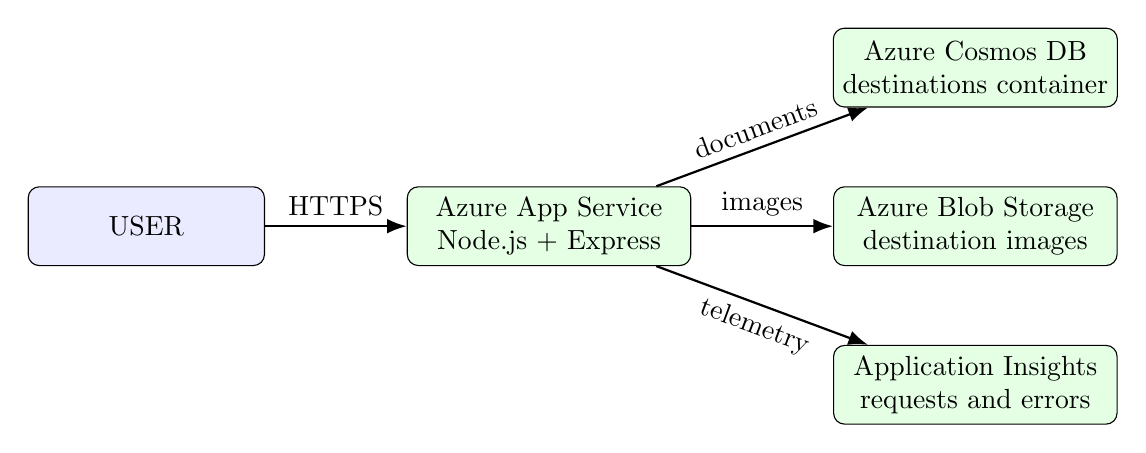
\begin{tikzpicture}[
  node distance=1.0cm and 1.8cm,
  box/.style={draw, rounded corners, align=center,
              minimum width=3.0cm, minimum height=1cm, fill=blue!8},
  service/.style={draw, rounded corners, align=center,
                  minimum width=3.6cm, minimum height=1cm, fill=green!10},
  arrow/.style={-{Latex[length=2.5mm]}, thick}
]
  % --- left column -------------------------------------------------
  \node[box] (user) {USER};

  % --- middle column -----------------------------------------------
  \node[service, right=of user] (app) {Azure App Service\\Node.js + Express};

  % --- right column (stacked vertically) ---------------------------
  \node[service, right=of app] (blob)     {Azure Blob Storage\\destination images};
  \node[service, above=of blob] (cosmos)  {Azure Cosmos DB\\destinations container};
  \node[service, below=of blob] (insights){Application Insights\\requests and errors};

  % --- arrows -------------------------------------------------------
  \draw[arrow] (user) -- node[above] {HTTPS} (app);

  \draw[arrow] (app) -- node[above, sloped] {documents} (cosmos);
  \draw[arrow] (app) -- node[above]         {images}    (blob);
  \draw[arrow] (app) -- node[below, sloped] {telemetry} (insights);
\end{tikzpicture}
\end{center}

\section{Feature Integration}

Public cloud features were integrated into the application:\\ 1. Azure Blob Storage\\ 2. Application Insights\\ Both features are connected to the Node.js backend through environment variables configured in Azure App Service.

% \section{Features Added:}

\subsection{Azure Blob Storage}
The add destination form accepts a JPG, PNG, or WEBP image up to 5 MB. The server uploads the image to the \texttt{destination-images} Blob Storage container and stores the image URL with the destination document.

Blob Storage is useful because users can add a real image to a destination, which makes the catalogue more informative. It is designed for image and file storage, keeps image data separate from the Cosmos DB documents, and allows images to be served independently.

\subsection{Application Insights}
Application Insights collects HTTP request, dependency, and error information from the application. It is useful for checking the health of the public application, viewing user requests, and finding problems after deployment.

\section{Web app repo files}

\begin{tabular}{>{\ttfamily}p{0.30\textwidth} p{0.60\textwidth}}
\toprule
File \\
\midrule
server.js & Express server, API routes, validation, Cosmos DB, Blob Storage, and monitoring \\
public/index.html & Page structure, filters, cards, and add destination form \\
public/styles.css & Page design, layout, responsive styling, and animations \\
public/app.js & Loading, filtering, form submission, image upload, and error messages \\
data.json & Local development data \\
package.json & Project commands and dependencies \\
.github/workflows/ & GitHub Actions deployment workflow \\
\bottomrule
\end{tabular}

\section{Deployment}

The repository is connected to Azure App Service through GitHub Actions. When code is pushed to the main branch, the workflow installs the Node.js dependencies and deploys the application to Azure.

The Azure App Service environment variables are:

\begin{verbatim}
COSMOS_ENDPOINT
COSMOS_KEY
COSMOS_DATABASE=travelCatalogue
COSMOS_CONTAINER=destinations
AZURE_STORAGE_CONNECTION_STRING
AZURE_STORAGE_CONTAINER=destination-images
APPLICATIONINSIGHTS_CONNECTION_STRING
\end{verbatim}

The application was deployed successfully using Azure and is available at public URL in Section 2.

% \section{Testing}

% The following tests were completed:

% \begin{itemize}
%   \item The public application loads in a browser.
%   \item Existing destinations are displayed.
%   \item A new destination can be added.
%   \item Search and filters return matching destinations.
%   \item Invalid input displays an error instead of crashing the application.
%   \item Images can be uploaded when Blob Storage is configured.
%   \item Destinations are stored in Cosmos DB when Azure settings are configured.
%   \item GitHub Actions completes the build and deployment process successfully.
% \end{itemize}

% \section{Cost Control}

% The application uses the Azure for Students subscription. The App Service can be stopped when the application is not being graded and started again before the public URL. Unused Azure resources should be deleted after the assignment is complete.

\section{Requirement Mapping}

\begin{tabular}{p{0.38\textwidth} p{0.52\textwidth}}
\toprule
Assignment requirement & Implementation \\
\midrule
Data layer & Azure Cosmos DB for NoSQL \\
Add entries & Add destination form and \texttt{POST /api/destinations} \\
List entries & Catalogue page and \texttt{GET /api/destinations} \\
Filter attributes & Search, continent, travel mood, and daily budget \\
Invalid inputs & Server-side validation and form error messages \\
Public URL & Azure App Service HTTPS URL \\
Two cloud features & Azure Blob Storage and Application Insights \\
Documentation & This PDF report and the project README \\
\bottomrule
\end{tabular}

\section{Conclusion}

Here a Web app custom named: U-AT\_lasTravel meets the requirements for a public cloud travel catalogue. It uses Azure Cosmos DB as a cloud data layer, Azure App Service for public hosting, Azure Blob Storage for images, and Application Insights for monitoring.

\end{document}
